% Options for packages loaded elsewhere
\PassOptionsToPackage{unicode}{hyperref}
\PassOptionsToPackage{hyphens}{url}
%
\documentclass[
  12pt,
  a4paper]{extarticle}
\title{Analysis 1B --- Tutorial 8}
\author{Christian Jones: University of Bath}
\date{March 2023}

\usepackage{amsmath,amssymb}
\usepackage{lmodern}
\usepackage{iftex}
\ifPDFTeX
  \usepackage[T1]{fontenc}
  \usepackage[utf8]{inputenc}
  \usepackage{textcomp} % provide euro and other symbols
\else % if luatex or xetex
  \usepackage{unicode-math}
  \defaultfontfeatures{Scale=MatchLowercase}
  \defaultfontfeatures[\rmfamily]{Ligatures=TeX,Scale=1}
\fi
% Use upquote if available, for straight quotes in verbatim environments
\IfFileExists{upquote.sty}{\usepackage{upquote}}{}
\IfFileExists{microtype.sty}{% use microtype if available
  \usepackage[]{microtype}
  \UseMicrotypeSet[protrusion]{basicmath} % disable protrusion for tt fonts
}{}
\makeatletter
\@ifundefined{KOMAClassName}{% if non-KOMA class
  \IfFileExists{parskip.sty}{%
    \usepackage{parskip}
  }{% else
    \setlength{\parindent}{0pt}
    \setlength{\parskip}{6pt plus 2pt minus 1pt}}
}{% if KOMA class
  \KOMAoptions{parskip=half}}
\makeatother
\usepackage{xcolor}
\IfFileExists{xurl.sty}{\usepackage{xurl}}{} % add URL line breaks if available
\IfFileExists{bookmark.sty}{\usepackage{bookmark}}{\usepackage{hyperref}}
\hypersetup{
  pdftitle={Analysis 1B --- Tutorial 8},
  pdfauthor={Christian Jones: University of Bath},
  hidelinks,
  pdfcreator={LaTeX via pandoc}}
\urlstyle{same} % disable monospaced font for URLs
\usepackage[margin=2.5cm]{geometry}
\usepackage{longtable,booktabs,array}
\usepackage{calc} % for calculating minipage widths
% Correct order of tables after \paragraph or \subparagraph
\usepackage{etoolbox}
\makeatletter
\patchcmd\longtable{\par}{\if@noskipsec\mbox{}\fi\par}{}{}
\makeatother
% Allow footnotes in longtable head/foot
\IfFileExists{footnotehyper.sty}{\usepackage{footnotehyper}}{\usepackage{footnote}}
\makesavenoteenv{longtable}
\usepackage{graphicx}
\makeatletter
\def\maxwidth{\ifdim\Gin@nat@width>\linewidth\linewidth\else\Gin@nat@width\fi}
\def\maxheight{\ifdim\Gin@nat@height>\textheight\textheight\else\Gin@nat@height\fi}
\makeatother
% Scale images if necessary, so that they will not overflow the page
% margins by default, and it is still possible to overwrite the defaults
% using explicit options in \includegraphics[width, height, ...]{}
\setkeys{Gin}{width=\maxwidth,height=\maxheight,keepaspectratio}
% Set default figure placement to htbp
\makeatletter
\def\fps@figure{htbp}
\makeatother
\setlength{\emergencystretch}{3em} % prevent overfull lines
\providecommand{\tightlist}{%
  \setlength{\itemsep}{0pt}\setlength{\parskip}{0pt}}
\setcounter{secnumdepth}{5}
\newcommand{\BOO}{BOO}
\usepackage {hyperref}
\hypersetup {colorlinks = true, linkcolor = blue, urlcolor = blue}
\usepackage{float}
\ifLuaTeX
  \usepackage{selnolig}  % disable illegal ligatures
\fi

\usepackage{amsthm}
\theoremstyle{plain}
\newtheorem*{theorem*}{Theorem}\newtheorem{theorem}{Theorem}[section]
\theoremstyle{definition}
\newtheorem*{definition*}{Definition}\newtheorem{definition}{Definition}[section]
\theoremstyle{plain}
\newtheorem*{proposition*}{Proposition}\newtheorem{proposition}[theorem]{Proposition}
\newtheorem*{Definitions*}{Definitions}\newtheorem{Definitions}[definition]{Definitions}
\theoremstyle{plain}
\newtheorem*{lemma*}{Lemma}\newtheorem{lemma}{Lemma}[section]
\theoremstyle{plain}
\newtheorem*{corollary*}{Corollary}\newtheorem{corollary}{Corollary}[section]
\theoremstyle{plain}
\newtheorem*{conjecture*}{Conjecture}\newtheorem{conjecture}{Conjecture}[section]
\theoremstyle{definition}
\newtheorem*{example*}{Example}\newtheorem{example}{Example}[section]
\theoremstyle{definition}
\newtheorem*{exercise*}{Exercise}\newtheorem{exercise}{Exercise}[section]
\newtheorem*{Thought*}{Thought}\newtheorem{Thought}{Thought}[section]
\theoremstyle{remark}
\newtheorem*{remark*}{Remark}
\newtheorem*{solution*}{Solution}
\newtheorem*{Example*}{Example}
\theoremstyle{remark}
\newtheorem*{Proof*}{Proof}
\newtheorem*{Examples*}{Examples}
\let\BeginKnitrBlock\begin \let\EndKnitrBlock\end


%\usepackage[english,shorthands=off]{babel}
\usepackage{etoolbox}
\usepackage{spverbatim}
\makeatletter
\@ifpackageloaded{float}{}{\usepackage{float}}
\@ifpackageloaded{adjustbox}{}{\usepackage[Export]{adjustbox}}
\makeatother
\floatplacement{figure}{H}
\newcommand{\scalefactor}{1.2}
\adjustboxset*{min width=\scalefactor\width,max width=\linewidth}
\renewcommand{\familydefault}{phv}
\fontfamily{phv}\selectfont
\renewcommand{\em}{\bf}\renewcommand{\textit}{\textbf}\renewcommand{\emph}{\textbf}\renewcommand{\it}{\bf}\renewcommand{\itshape}{\bf}
\setlength{\parindent}{0.0pt}
\setlength{\parskip}{1.0\baselineskip}
\renewcommand{\baselinestretch}{1.5}\selectfont
\setlength{\mathsurround}{0.2em}
\setlength{\arraycolsep}{0.5cm}\renewcommand{\arraystretch}{1.5}
\addtolength{\jot}{\baselineskip}
\renewcommand{\;}{\,}
\sloppy
\allowdisplaybreaks
\usepackage{amsthm}
\newtheoremstyle{plain}{20pt}{3pt}{}{}{\bfseries}{.\newline\nobreak}{1.0em\nobreak}{}
\newtheoremstyle{definition}{20pt}{3pt}{}{}{\bfseries}{.\newline\nobreak}{1.0em\nobreak}{}
\newtheoremstyle{remark}{20pt}{3pt}{}{}{\bfseries}{.\newline\nobreak}{1.0em\nobreak}{}
\csundef{Proof}
\csundef{endProof}
\newenvironment{Proof}
  {\noindent{\bf Proof.}\hspace*{1em}}% Begin
  {\qed\par}% End
%% When redefining an environment it is vital that it has 
%% the same number of arguments as the original
\renewenvironment{proof}[1][\proofname]
  {\trivlist\item\relax\noindent{\bf {#1}.}\hspace*{1em}}% Begin
  {\qed\endtrivlist}% End

\begin{document}
\maketitle

{
\setcounter{tocdepth}{2}
\tableofcontents
}
\newpage
\pagenumbering{arabic}

\hypertarget{introduction}{%
\section*{Introduction}\label{introduction}}
\addcontentsline{toc}{section}{Introduction}

Here is the material to accompany the 8th Analysis 1B Tutorial on the 27th March. Alternative formats can be downloaded by clicking the download icon at the top of the page. Please send any comments or corrections to \href{mailto:caj50@bath.ac.uk}{Christian Jones (caj50)}. To return to the homepage, click \href{http://caj50.github.io/tutoring.html}{here}.

\hypertarget{lecture-recap}{%
\section{Lecture Recap}\label{lecture-recap}}

This week, we look at some of the consequences of the Mean Value Theorem! These include a method of calculating limits (L'Hôpital's Rule) and a method of approximating functions (Taylor's Theorem). Throughout all of this, we are going to need functions which are at least twice differentiable, and along the way, we will develop some conditions to classify extrema.

\hypertarget{lhuxf4pitals-rule-1}{%
\subsection[L'Hôpital's Rule ]{\texorpdfstring{L'Hôpital's Rule \footnote{Or if you prefer your 17th Century French, de L'Hospital's rule.}}{L'Hôpital's Rule }}\label{lhuxf4pitals-rule-1}}

Suppose we want to calculate the limit \[\lim_{x \to 3} \frac{x^2 - 9}{x - 3} = L.\] Using sequences, say, we can easily show that \(L = 6\), but why don't we use the algebra of limits? After all, we formulated AoL to make our lives easier, and both \(\lim_{x \to 3} x^2 - 9\) and \(\lim_{x \to 3} x - 3\) exist. The issue is that if we naïvely apply AoL, we end up running into an \emph{indeterminate form}. This is an object of the form \[\frac{0}{0} \; \text{or} \; \frac{\infty}{\infty},\] and is named as such because we cannot assign a value to it. For more complicated limits, we could really use a method which can help us in the cases where an indeterminate form arises. Such a method exists, and is known as L'Hôpital's rule\footnote{It's worth mentioning that there are many different statements of this rule. The one given here combines Theorem 2.32 from the lecture notes (which is L'Hôpital for right-handed limits) with a corresponding statement for left-handed limits.}:

\BeginKnitrBlock{theorem}[L'Hôpital's Rule]
{\label{thm:thm1} }Let \(c, L \in \mathbb{R}\), \(\eta > 0\), \(D = (c-\eta, c + \eta)\setminus\lbrace c \rbrace,\) and let \(f,g: D \to \mathbb{R}\) be differentiable on \(D\). Furthermore, suppose that:

\begin{itemize}
\item
  \(\lim_{x \to c} f(x) = 0 = \lim_{x \to c} g(x)\)
\item
  \(g'(x) \neq 0 \;\; \forall x \in D,\) and
\item
  \(\lim_{x \to c} \frac{f'(x)}{g'(x)}\) exists.
\end{itemize}

Then \(\lim_{x \to c} \frac{f(x)}{g(x)} = \lim_{x \to c} \frac{f'(x)}{g'(x)}.\)
\EndKnitrBlock{theorem}

\hypertarget{higher-order-derivatives}{%
\subsection{Higher Order Derivatives}\label{higher-order-derivatives}}

\BeginKnitrBlock{definition}[Higher Order Derivatives]
{\label{def:def1} }Let \(a,b \in \mathbb{R}\) with \(a < b\), and \(f:(a,b) \to \mathbb{R}\). We say that \(f\) is \(n\)-times differentiable at \(c \in (a,b)\) if:

\begin{itemize}
\item
  \(n=1\): \(\lim_{x \to c}\frac{f(x) - f(c)}{x - c}\) exists.
\item
  \(n>1\): There exists \(\delta \in (0, b-a)\) such that \(f\) is \(n\)-times differentiable on \((c - \delta, c + \delta)\) and the \((n-1)\)-th derivative function of \(f\), \(f^{(n-1)}: (c - \delta, c + \delta) \to \mathbb{R}\) is differentiable at \(c\).
\end{itemize}
\EndKnitrBlock{definition}

In terms of notation, we have that \[f^{(n)}(x) = \left(f^{(n-1)}\right)'(x) =  f^{\hspace{-0.2cm}\overbrace{\,'\cdots'\,}^{n\; \text{primes}}}\hspace{-0.25cm}(x).\] The inclusion of brackets here to specify a derivative is really important, as omitting them just gives us \(f^n\), which is the product of \(f\) with itself \(n\) times!

As you've seen, polynomials, \(\sin\), \(\cos\) and \(\exp\) are \(n\)-times differentiable on \(\mathbb{R}\) for all \(n \in \mathbb{N}\). These functions are known as smooth. As a result, the function \(f:\mathbb{R} \to \mathbb{R}\) given by \[f(x) = \lvert x \rvert \frac{x^n}{(n+1)!}\] can be differentiated infinitely many times on \(\mathbb{R}\setminus\lbrace 0 \rbrace\), but only \(n\) times at \(x = 0\).

\hypertarget{conditions-for-extrema}{%
\subsubsection{Conditions for Extrema}\label{conditions-for-extrema}}

Second order derivatives in particular can be quite useful when looking at the extrema of functions. Given a set of candidate extrema (critical points and interval endpoints), we can use the second derivatives to establish some selection criteria to determine whether they are local max or local min points.

Here, we present the results for local max points of a function \(f\) only, as corresponding results for local min points can be deduced by considering \(-f\).

\BeginKnitrBlock{theorem}[Necessary Conditions for Local Maxima]
{\label{thm:thm2} }Let \(a,b \in \mathbb{R}\) with \(a<b\). Also, let \(p \in (a,b)\), and let \(f: (a,b) \to \mathbb{R}\) be differentiable on \((a,b)\) and twice differentiable at \(p\). If \(p\) is a local max point of \(f\), then \(f'(p) = 0\), and \(f''(p) \leq 0\).
\EndKnitrBlock{theorem}

One thing to note here is that this theorem allows you to discount points from being local maxima --- you cannot use it to say that a point is a local maximum point! To do that, you need the converse of this theorem to hold true, and by considering the function \(f:(-1,1) \to \mathbb{R}\), \(f(x) = x^3\) at \(p=0\), we see that the converse does not hold.

However, all hope is not lost! A partial converse does hold, which we can use to determine whether a point is a local maximum:

\BeginKnitrBlock{theorem}[Sufficient Conditions for Local Maxima]
{\label{thm:thm3} }Let \(a,b \in \mathbb{R}\) with \(a<b\). Also, let \(p \in (a,b)\), and let \(f: (a,b) \to \mathbb{R}\) be differentiable on \((a,b)\) and twice differentiable at \(p\). If \(f'(p) = 0\), and \(f''(p) < 0\), then \(p\) is a local max point of \(f\).
\EndKnitrBlock{theorem}

\hypertarget{taylors-theorem}{%
\subsection{Taylor's Theorem}\label{taylors-theorem}}

This next theorem is quite possibly the most useful\footnote{In a practical sense, anyway.} theorem that you'll learn in this course. Simply put, it gives you a way of approximating a complicated function by a polynomial. In maths terms, we have the following:

\BeginKnitrBlock{theorem}[Taylor's Theorem]
{\label{thm:thm4} }Let \(n \in \mathbb{N}\) and \(x_0,x \in \mathbb{R}.\) Let \(I \subseteq \mathbb{R}\) be an open interval containing \([x_0,x].\) Let \(f:I\to\mathbb{R}\) be \((n+1)\)-times differentiable on \(I\). Then, \(\exists c \in (x_0,x)\) such that \[f(x) = \sum_{k = 0}^{n} \frac{f^{(k)}(x_0)}{k!}(x - x_0)^k + R_n,\] where \[R_n = \frac{f^{(n+1)}(c)}{(n+1)!}(x - x_0)^{n+1}.\]
\EndKnitrBlock{theorem}

Here, \(R_n\) is a remainder term, and the form above is known as the \emph{Lagrange form} of the remainder\footnote{There is another form, which you may not be surprised to learn is named after Cauchy.}. As an example, we can plot successive Taylor approximations to \(\sin\), as is seen in Figure \ref{fig:sinapx} (Taken from \href{By\%20IkamusumeFan\%20-\%20Own\%20work,\%20CC\%20BY-SA\%203.0,\%20https://commons.wikimedia.org/w/index.php?curid=27865201}{Wikipedia}). What we find is that even small term Taylor approximations can be quite accurate!

\begin{figure}

{\centering 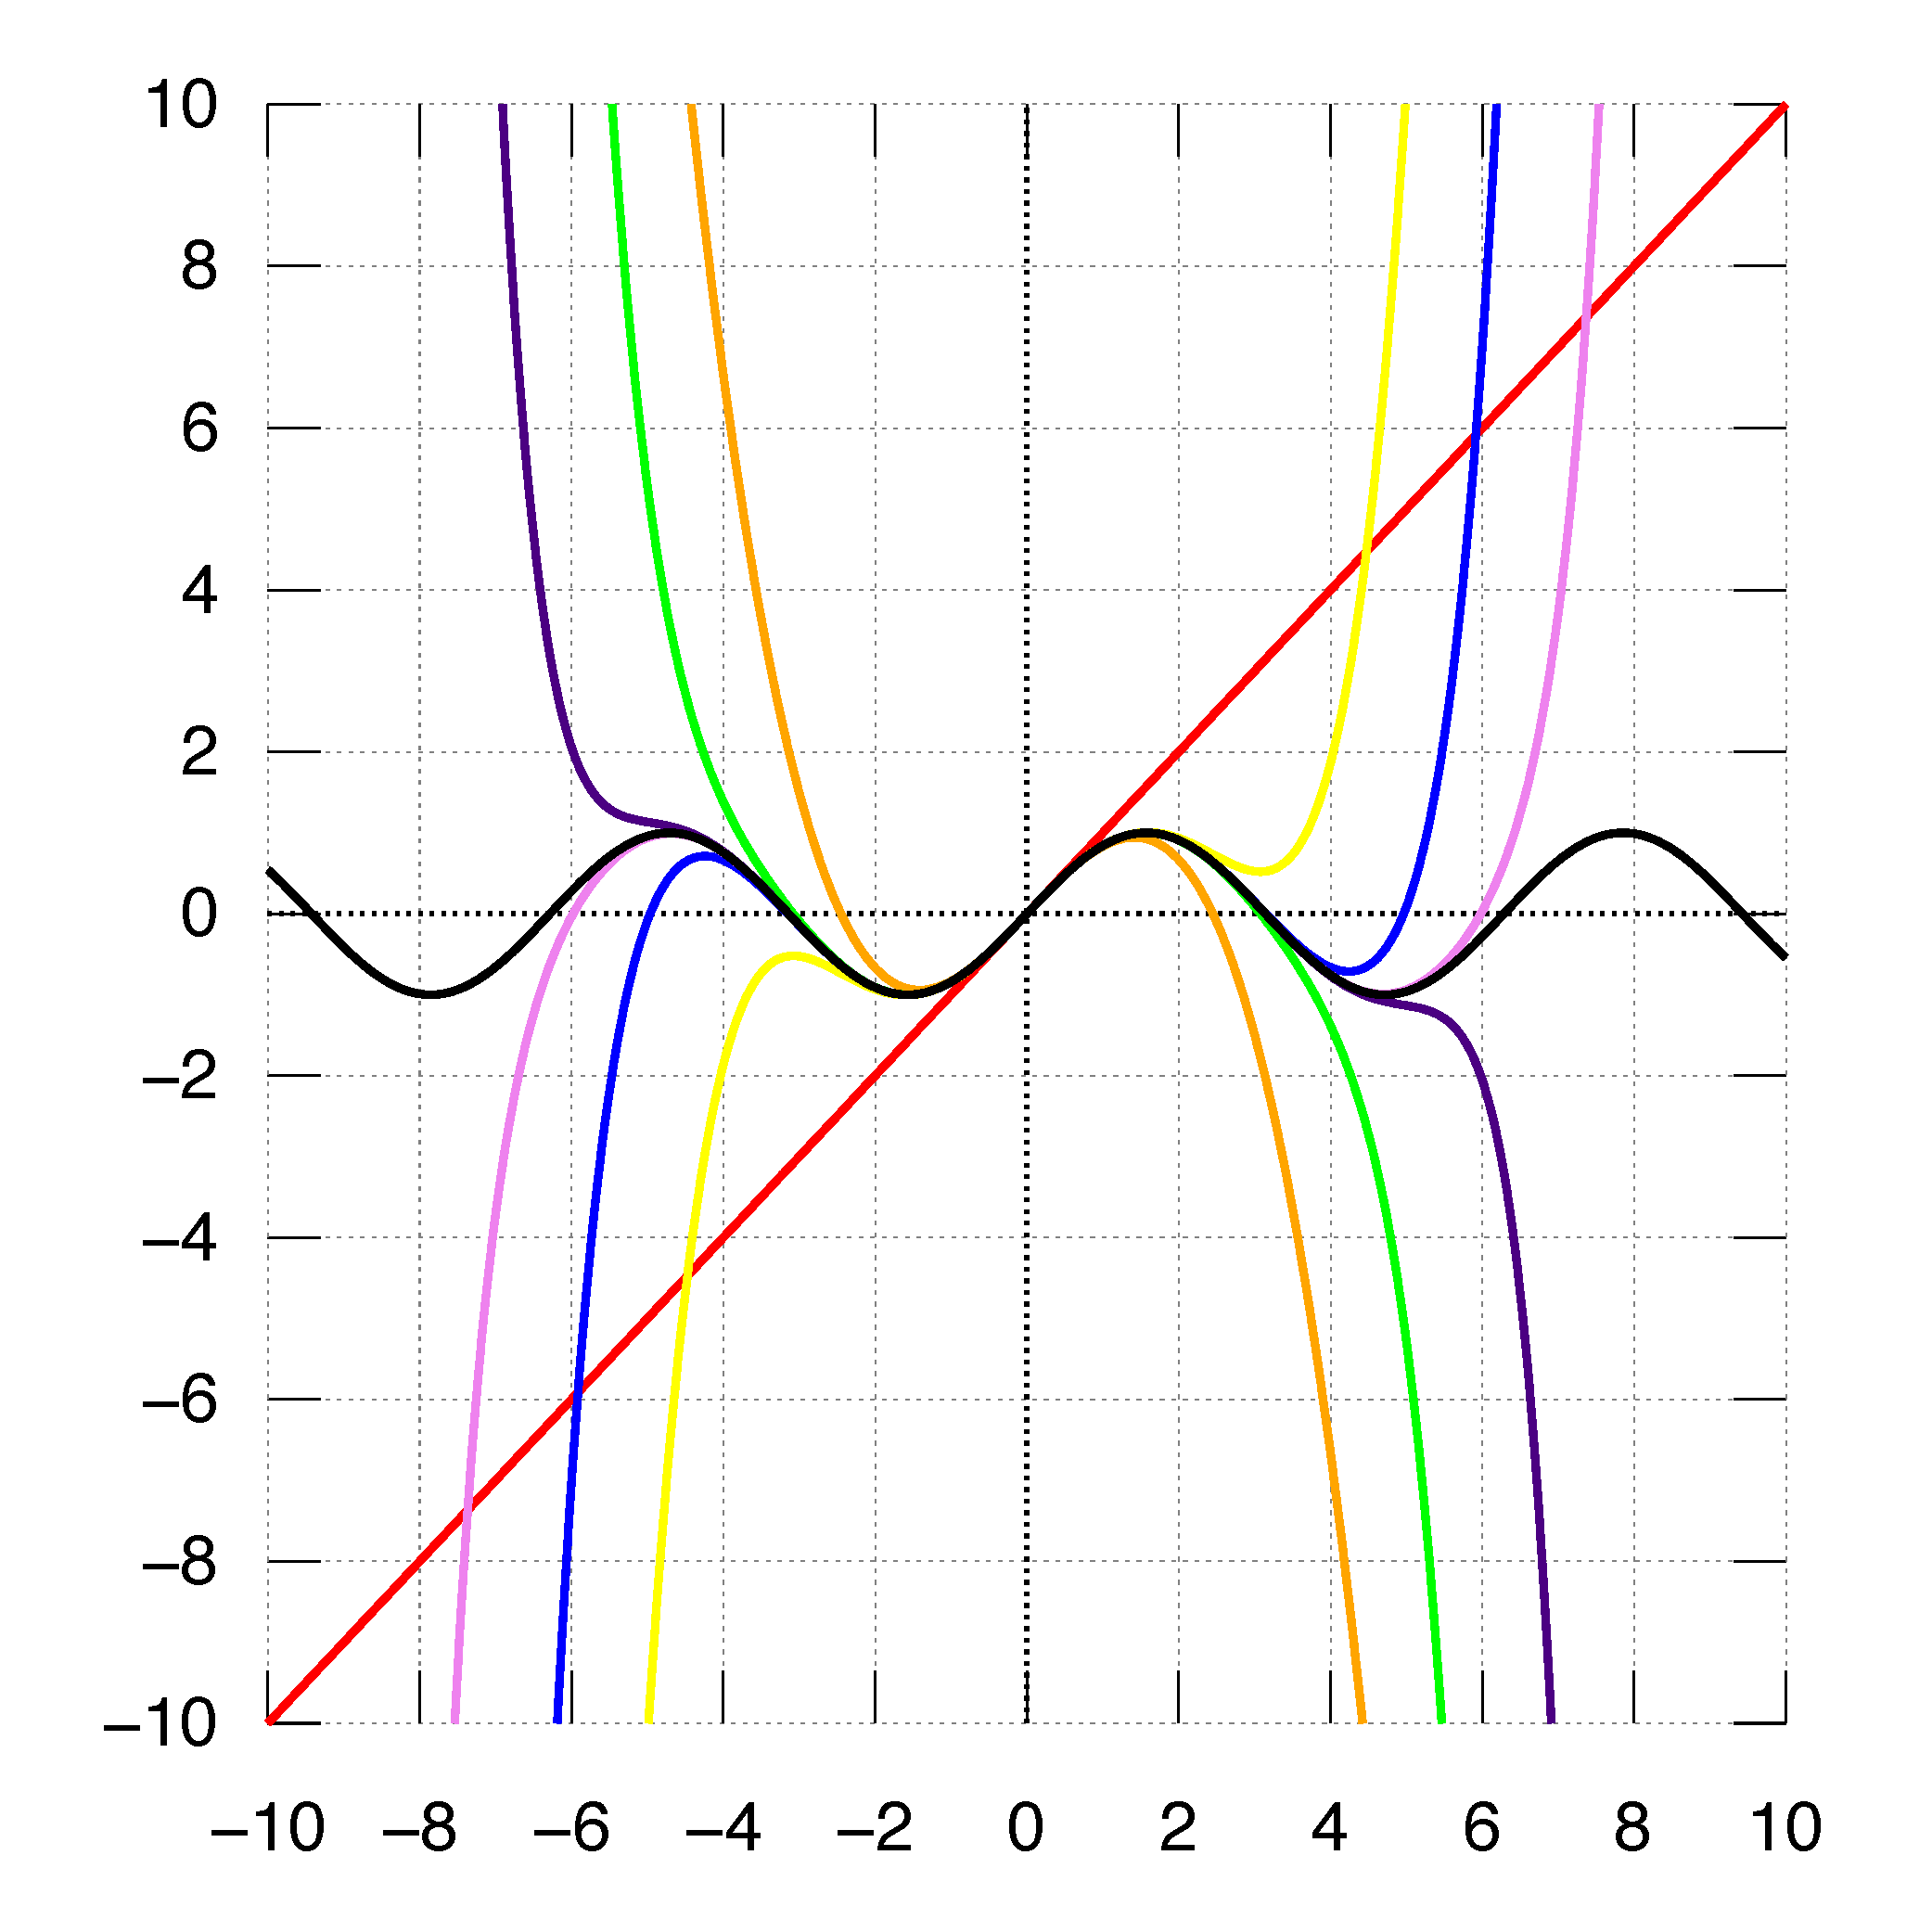
\includegraphics[width=\Width,height=\Height]{sinapx} 

}

\caption{Taylor approximations to $\sin(x)$ at $x=0$ of degree 1 (red), 3 (orange), 5 (yellow), 7 (green), 9 (blue), 11 (purple) and 13 (pink).}\label{fig:sinapx}
\end{figure}

So, why is this theorem so useful? Firstly, it allows computers to work with complicated, non-linear functions such as \(\exp\) and \(\sin\) without losing too much by way of accuracy. Secondly, Taylor's theorem allows us to actually do some analysis on physical systems.

\BeginKnitrBlock{example}
{\label{exm:ex1} }Consider a pendulum consisting of a mass \(m\) connected to a string (under tension) of length \(\ell\).

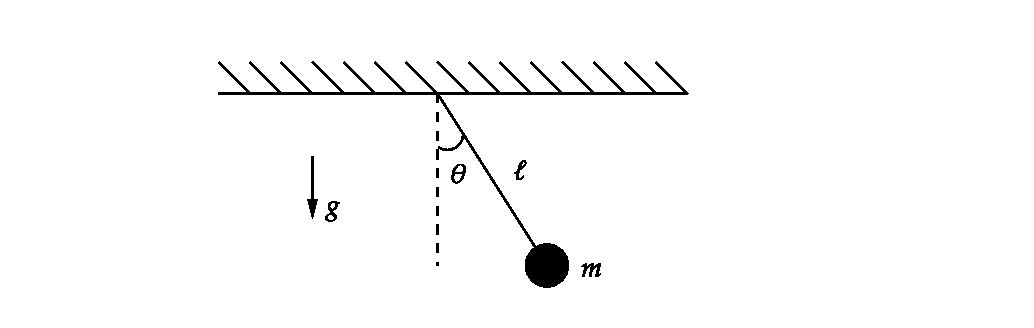
\includegraphics[width=\Width,height=\Height]{./bob.pdf}

If you've seen it in MA10236 (Vectors, Vector Calculus and Mechanics), the equation of motion for this system is given by \[\theta'' + \frac{g}{\ell}\sin(\theta) = 0.\] This is a non-linear differential equation, which we need to solve numerically. However, if we make a `small angle' approximation, then by Taylor's theorem, \(\sin(\theta) \approx \theta\), and the equation becomes \[\theta'' + \frac{g}{\ell}\theta= 0.\] This is analytically tractable, and --- subject to suitable initial conditions --- we can write down a solution!
\EndKnitrBlock{example}
Finally, we can also use the expansion in Taylor's Theorem to define differentiation in more than one dimension! If you're interested in how this is done, take \href{https://people.bath.ac.uk/mo221/MA20219/notes.bho/lecturenotes.pdf}{MA20219} (Analysis 2B) next year!\footnote{The link here will take you to some lecture notes; see Chapter 1 for details.}

\hypertarget{hints}{%
\section{Hints}\label{hints}}

As per usual, here's where you'll find the problem sheet hints!

\begin{enumerate}
\def\labelenumi{\arabic{enumi})}
\tightlist
\item
  Proof by induction comes to mind here. Make sure you justify the important steps in the proof using course results too!
\item
  `Tutorial Question 2' from this week's tutorial should help. I think there might be an example in the lecture notes as well.
\item
  Since integration has been banned, you'll have to find another way to relate \(g\) to its first and second derivatives. There's a theorem from this week that'll certainly help!
\end{enumerate}

\end{document}
